%%%%%%%%%%%%%%%%%%%%%%%%%%%%%%%%%%%%%%%%%%%%%%%%%%%%%%%%%%%%%%%%%%%%%
% LaTeX Template: Project Titlepage Modified (v 0.1) by rcx
%
% Original Source: http://www.howtotex.com
% Date: February 2014
% 
% This is a title page template which be used for articles & reports.
% 
% This is the modified version of the original Latex template from
% aforementioned website.
% 
%%%%%%%%%%%%%%%%%%%%%%%%%%%%%%%%%%%%%%%%%%%%%%%%%%%%%%%%%%%%%%%%%%%%%%

\documentclass[11pt,a4paper]{article}
\usepackage[T1]{fontenc}
\AtBeginDocument{\usefont{\encodingdefault}{phv}{m}{n}}
\usepackage{helvet}
\usepackage{fullpage}
\usepackage[table,xcdraw]{xcolor}
\usepackage{fancyhdr}
\pagestyle{fancy}
\lhead{}
\setlength{\headsep}{0.3in}
\setlength\parindent{0pt}
\setlength{\parskip}{1em}
\usepackage[english]{babel}
\usepackage{amsmath}
\usepackage{siunitx}
\usepackage{graphicx}
\usepackage[colorinlistoftodos]{todonotes}
\usepackage{subfig}
%\usepackage{subcaption}
\usepackage[export]{adjustbox}[2011/08/13]
\usepackage[nottoc,numbib]{tocbibind}
\usepackage{float}
\usepackage{eurosym}
\usepackage{gensymb}
\usepackage{wrapfig}
\usepackage{multirow}
\usepackage[toc,page]{appendix}
\usepackage{hyperref}
\usepackage[all]{hypcap}
\lhead{{\small Ismaeel Zaman }}
\chead{{\small AVDASI4 FEDR - Weight and Balance, Stability \& Control}}
\rhead{
\includegraphics[height=5mm]{Logo.png}}
\cfoot{\thepage}
\renewcommand{\headrulewidth}{1pt}
\usepackage[margin=2cm]{geometry}
\usepackage{titlesec}
\titlespacing{\section}{0pt}{5pt}{4pt}
\titlespacing{\subsection}{0pt}{5pt}{4pt}
\titlespacing{\subsubsection}{0pt}{5pt}{4pt}
\def\therefore{{\tiny$\bullet$}\kern-0.2ex\raisebox{1ex}{\tiny$\bullet$}\kern-0.2ex{\tiny$\bullet$}}
%-------------------------------------------------------------------------------
% TITLE PAGE
%-------------------------------------------------------------------------------

\begin{document}
\begin{titlepage}

\begin{figure}[H]
\minipage{0.32\textwidth}
  
\includegraphics[width=.75\linewidth]{University_of_Bristol_logo.png}
  \endminipage\hfill
  \minipage{0.32\textwidth}
  \centering
    
\includegraphics[width=.75\linewidth]{Logo.png}
    \endminipage\hfill
    \minipage{0.32\textwidth}%
    \hspace{12mm}
      \includegraphics[width=.75\linewidth]{Aero_logo.png}
      \endminipage
      \end{figure}

\center 
\hrule
\textsc{\Large \textbf{Aerospace Vehicle Design \& System Integration 4 \\ \vspace{2mm} Final Engineering Definition Report}}

{ \large  Weight and Balance, Stability \& Control }
\vspace{6pt}
\hrule

\textsc{\textbf{Ismaeel Zaman}} 


\textsc{\textbf{Academic Advisor:} Professor Nick Lieven} \\
\textsc{\textbf{PG Advisor:} Harry Felton}
\\[0.5cm]
\textsc{\large \today} 
\vspace{6pt}

\hrule
\vspace{10mm}


\textbf{Abstract:}
\\
words words words words words words words words words words words words words words words words words words  words words words words words words words words words  words words words words words words words words words  words words words words words words words words words  words words words words words words words words words  words words words words words words words words words  words words words words words words words words words  words words words words words words words words words  words words words words words words words words words  words words words words words words words words words   

\begin{figure}[H]
    \centering
        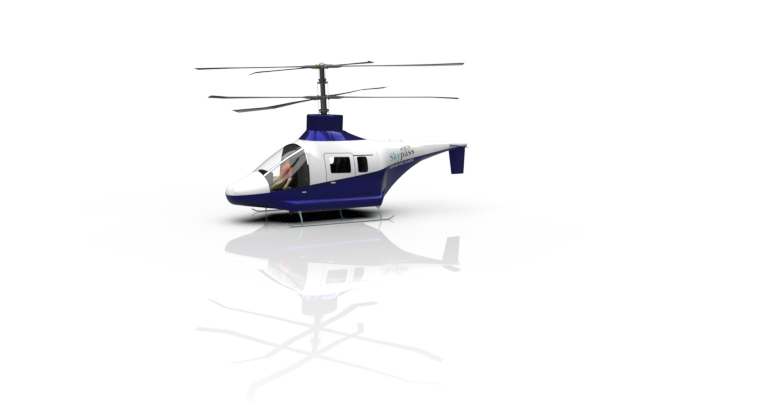
\includegraphics[width=0.5\textwidth]{High_res_2.png}
        \end{figure}
\hrule


\vfill
\end{titlepage}
\newpage
\tableofcontents
\thispagestyle{empty}
\newpage
\listoftables
\thispagestyle{empty}
\listoffigures
\thispagestyle{empty}
\newpage
NOMENCLATURE
\thispagestyle{empty}
\newpage
\setcounter{page}{1}
%-------------------------------------------------------------------------------
% Section title formatting
%\sectionfont{\scshape}
%-------------------------------------------------------------------------------

%-------------------------------------------------------------------------------
% BODY
%-------------------------------------------------------------------------------

\section{Introduction}
% •	Overview of group project
% •	Describe my technical role, the heading, overall responsibility
% •	Areas of Technical input (requirements)
% •	Describe Structure of report

\section{Technical Overview}
An overview of the design process for this specialisation can be seen in  Figure ADDREF.
\begin{figure}[H]
	\flushright
	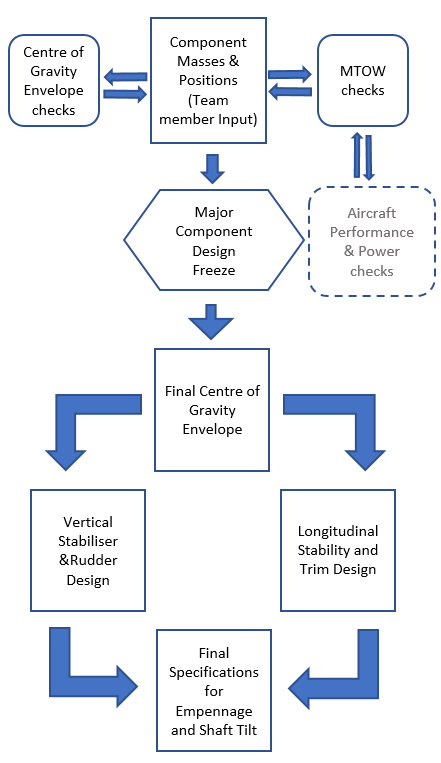
\includegraphics[width=0.4\textwidth]{Flowchart.PNG}
	\caption{Design process}
	\centering
	\label{fig:flowchart}
\end{figure}
% \begin{wrapfigure}[15]{r}{5.5cm}
%     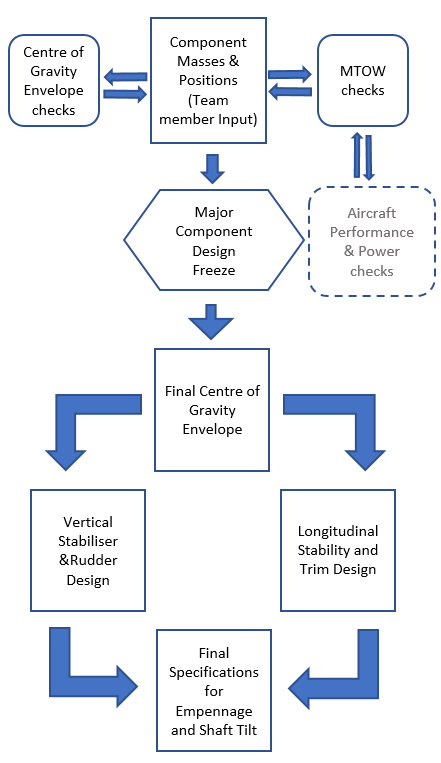
\includegraphics[width=5cm]{Flowchart.PNG}
%     \caption{A rotating parachute design for submunitions \cite{DOHERR1992Nine-degree-of-freedomSystems}}
%     \label{fig:doherr}
%     %\vspace{-510pt}
% \end{wrapfigure}
ggr
rrr
r
r
r
r
r
rr

rr
r
%INSERT FANCY FLOWCHART

\section{Mass Distribution}
\subsection{Mass Breakdown}
% Describe how mass considerations influenced design process.
% Table of mass breakdown, pie chart
% Passenger and luggage loadout. configurations. CG affected in 3D. Show CG V loading. Show 3D plot.
% Say that median CG location used for trim design so that passenger comfort at extreme loadouts.
The mass breakdown and key weights can be seen in Figure \ref{fig:pie} and Table \ref{tab:tabmass}. While the moments of inertia of the empty helicopter can be seen in Table \ref{tab:tabinertia}.
\begin{table}[H]
	\begin{minipage}{0.5\linewidth}
		\caption{Table of key weights}
		\label{tab:tabmass}
		\centering
\begin{tabular}{cc}
    \hline
    \rowcolor[HTML]{DAE8FC} 
    Weights       & kg   \\ \hline
    MTOW          & 2730 \\ \hline
    OWE+Batteries & 2180 \\ \hline
    MZFW          & 1070 \\ \hline
\end{tabular}
\vspace{10pt}
\caption{Table of Moments of Inertia}
		\label{tab:tabinertia}
\begin{tabular}{cc}
\hline
\rowcolor[HTML]{DAE8FC} 
Moments of Inertia & kgm$^2$   \\ \hline
$I_{y_{CG}}$        & 3574.35 \\ \hline
$I_{x_{CG}}$        & 2455.47 \\ \hline
$I_{z_{CG}}$        & 1118.88 \\ \hline
\end{tabular}
	\end{minipage}\hfill
	\begin{minipage}{0.45\linewidth}
		\centering
		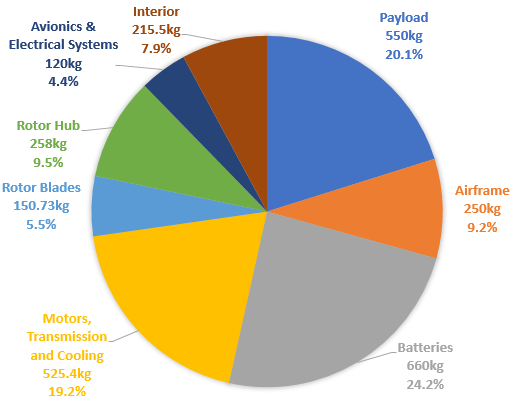
\includegraphics[width=\textwidth]{PIE.PNG}
		\captionof{figure}{Pie chart showing mass breakdown of components}
		\label{fig:pie}
	\end{minipage}
\end{table}
A more detailed breakdown can be seen in Appendix \ref{tab:massb}.
\subsection{Centre of Gravity Variation}
Following the finalisation of component masses and positions, the centre of gravity range, as it varies with payload loadout, was calculated in 3D. The assumptions were that each human being weighed 90kg, and each passenger had the option of carrying up to 25kg of luggage each. This formed the total payload mass of 550kg, set by JAR-OPS3. Every component was assumed to be a point mass. For every flight case the pilot was assumed present.
The longitudinal CG against AUW can be seen in Figure \ref{fig:CG1} and the 3D CG envelope can be seen in Figure \ref{fig:CG2}.

\begin{figure}[H]
\centering
\begin{minipage}{.5\textwidth}
  \centering
  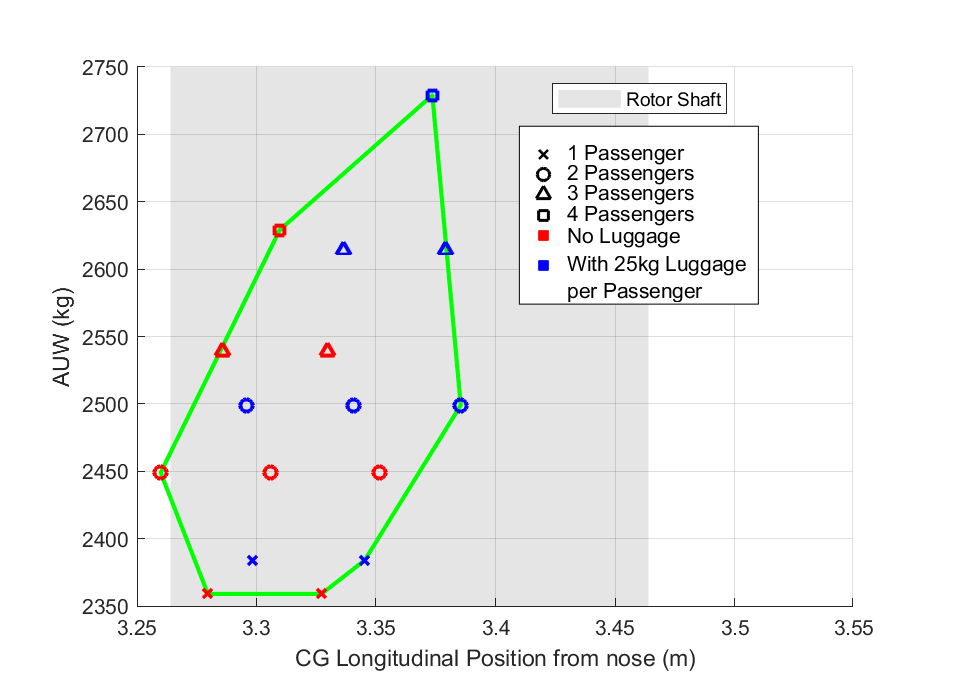
\includegraphics[width=\linewidth]{CGVAUW.eps}
  \captionof{figure}{Longitudinal CG versus AUW}
  \label{fig:CG1}
\end{minipage}%
\begin{minipage}{.5\textwidth}
  \centering
  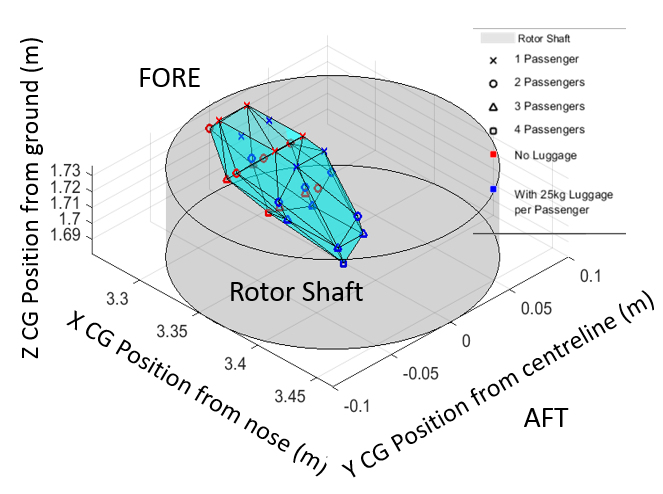
\includegraphics[width=\linewidth]{3D.PNG}
  \captionof{figure}{3D CG Envelope}
  \label{fig:CG2}
\end{minipage}
\end{figure}

Lateral and vertical CG envelopes can be seen in Appendix \ref{fig:CGlat}.
It was found that the CG location when empty lay 3mm forward of the centre of the main shaft and the largest deviation case consisted of 3 passengers, two in the front and one at the rear, without any luggage this is the leftmost point in Figure \ref{fig:CG1}. This resulted in a maximum deviation of 10.5cm forward of the main rotor, which is the preferred direction for stability \cite{prouty} and is relatively small. As can been seen in Figure \ref{fig:CG2}, in almost all cases the CG lies within the 20cm diameter rotor shaft.\\ This favourable CG envelope was a result of placing the heaviest components such as the gearbox, batteries and motors as close to the centre of the cabin as possible. During the design process it was evident that for structural reasons the main rotor would be better placed in the centre of the cabin, to achieve this the centre of mass had to be moved forward and so following a trade study, Appendix \ref{fig:batterypos}, the battery was moved under the floor of the cabin.

The CG range information was used to inform the design of the helicopter skids so as to satisfy the 12 degree inclination requirement. Following structural design and ground resonance considerations, which can be seen in the structures and rotor hub specialist reports respectively, the final skids allow for an on-ground inclination of 37.6 degrees. This is assuming worst case CG (empty).\\

\section{Shaft Tilt and Horizontal Stabiliser}

\subsection{Overview}
The aim of this section is to maximise passenger comfort and reduce power consumption through trim and empennage specifications.

Increasing passenger comfort can be done by minimising the fuselage pitch deviation from zero in both hover and cruise. Reducing power consumption can be done by minimising the flapping angles necessary.
\begin{figure}[H]
    \centering
    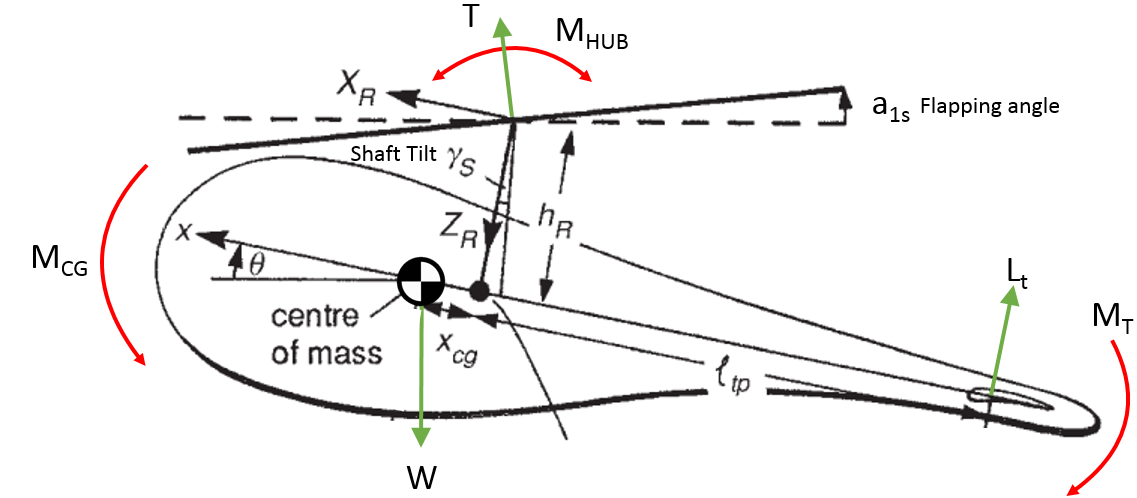
\includegraphics[width=0.8\textwidth]{FBD.PNG}
    \caption{Diagram showing key forces and moments}
    \label{fig:fbd}
\end{figure}{}
During forward flight the rotor must tilt forward to balance the forces generated by the drag of the fuselage.
In a standard helicopter with zero shaft tilt and an articulated hub the fuselage would also tilt forward slightly with the rotor disc, with the remainder of the tilt being fulfilled by the rotor flapping angle. 
However, large fuselage pitch angles are not very comfortable and so it is possible to have the rotor shaft fixed at a forward angle reduce fuselage pitch during cruise. This does have the drawback of increasing the fuselage pitch and flapping angle during hover and so a balance must be struck.

In addition, rotors with a blade hinge offset are able to impart moments onto the aircraft, this hub moment can be described by equation ADDREF. This is beneficial as it allows the aircraft to counter the moment created by not having a centre of mass exactly below the line of action of the rotor. This means it is able to force the fuselage to stay relatively parallel to the ground even in unfavourable CG conditions, much more so than if there was no hinge offset in which case the aircraft would simply tilt until the CG was directly under the main rotor. In this project, the hinge offset was calculated by the rotor blade and rotor hub specialists so as to reduce resonance and vibration. Details of its determination can be found in those reports.

This effect is mainly helpful during hover, where the only constraint is that the tip path plane of the rotor must remain parallel to the ground allowing the flapping angle to be adjusted to balance the moment from the CG offset, of course the resulting fuselage pitch is highly dependant on shaft tilt. In cruise, the tip path plane has the additional constraint of balancing of forward thrust and drag, meaning that the tip path plane is now angled forward. Now the resulting hub moment may only allow the fuselage to be 'corrected' to a certain degree, again dependant on shaft tilt, meaning that the pitch angle may not be ideal. \\
This is where the addition of a horizontal stabiliser is helpful. A horizontal stabiliser during cruise is able to generate a moment which can work in tandem with the moment of the rotor flapping angle to reduce fuselage pitch.

To summarise, the two aircraft specifications that need determining are the rotor shaft tilt ($\gamma$) and the moment generated by the horizontal stabiliser ($M_t$). The effect of these on the resulting fuselage pitch angles ($\theta$) in both hover and cruise, and the required flapping angles ($a_{1s}$) also in both hover and cruise need to be analysed and then a method of optimisation needs to be employed to obtain the best compromise of $\gamma$ and $M_t$.

Another layer of complexity arises when it becomes necessary to account for the varying location of CG for different payload configurations. Ensuring that the resulting characteristics of the aircraft are acceptable for all possible payload combinations is important as it must be able to remain viable in the varying situations it is likely to encounter being a public transport vessel.
\subsection{Assumptions}

The equations used for longitudinal stability and trim are adapted from Prouty \cite{prouty}, these equations are built on several assumptions:

\begin{itemize}
    \item Reverse flow region neglected.
    \item Tip loss and root cut out neglected.
    \item Small angles are assumed.
\end{itemize}{}

To simplify calculations further, additional assumptions have been made:

\begin{itemize}
    \item The rotor thrust vector is perpendicular to the tip path plane
    \item The two main 4-bladed rotors are assumed to flap in the same direction with equal magnitude therefore acts as a single rotor for trim purposes.
    \item Rotor downwash effects on drag of fuselage and empennage are ignored in calculations.
    \item Fuselage pitching moment and lift ignored.
    \item Minimum drag condition of fuselage assumed zero pitch.
\end{itemize}{}

In the absence of full CFD and/or wind tunnel testing, the aerodynamic characteristics of the fuselage have been ignored with the exception of flat plate drag, $D_f=1.84V^2$, this was obtained using conditions at cruise altitude.
The location of the horizontal stabiliser has been placed $5$ meters behind the centre of the cabin so that the downwash from the rotors would have a reduced affect. This means that the variable $M_t$ can be reduced to $L_t$ as $M_t=L_t\cdot l_t$. The coning angle of the rotors has been ignored as they do not produce a resultant moment that would affect trim.

The equations used can be seen in Appendix ADDREF\\

EQUATIONS HERE\\

A note on lateral stability and trim, unlike a penny-farthing a coaxial helicopter does not suffer from the lateral stability issues caused by the presence of a tail rotor, i.e side-slip, gust alleviation issues etc. Therefore, the lateral stability considerations are almost identical to that of longitudinal with the exception of that fact that the requirements in this direction are much reduced, CG positions change very little laterally and rotor flapping has no additional constraints either as the aircraft is not expected to fly sideways at any significant speed.
It can be said then that if the aircraft performs acceptably longitudinally then lateral stability should not be an issue as lateral flapping angles (flapping would be the aircraft's only way to exert lateral control) would be much less than longitudinal.

\subsection{Data Generation}
To be able to explore the relationships between the two input variables ($\gamma,L_t$) and the  four output variables ($a_{1s_{hover}},a_{1s_{cruise}},\theta_{f_{hover}},\theta_{f_{cruise}}$) for each CG position, a parameter sweep was performed.

The range of input values was a Shaft Tilt, $\gamma$, from $0$ to $-9$ degrees and a Tail lift, $L_t$ of $0$ to $900N$. This range was found to encompass the values of interest, i.e results that span across the zero angle planes, and also values that typical helicopters employ \cite{prouty}.

Initially the median CG position was used to obtain initial values and to allow sanity checks to be made. However, for any particular configuration of shaft tilt and tail force, the fuselage pitch angles and rotor flapping angles will change depending on the location of CG. Therefore, in order to obtain the maximum and minimum values that could be experienced by the aircraft each configuration had its full range of CG positions evaluated for with the maximum and minimum values for each configuration stored.

\subsection{Results}

The maximum and minimum values for pitch angles and flapping angles for both cruise and hover as CG is varied across its range were plotted against shaft angle and tail force. Two surface plots for cruise and two 2D plots for hover, as tail force has no effect on the hover condition, were produced. These can be seen below:

\begin{figure}[H]
\centering
\begin{minipage}{.48\textwidth}
  \centering
  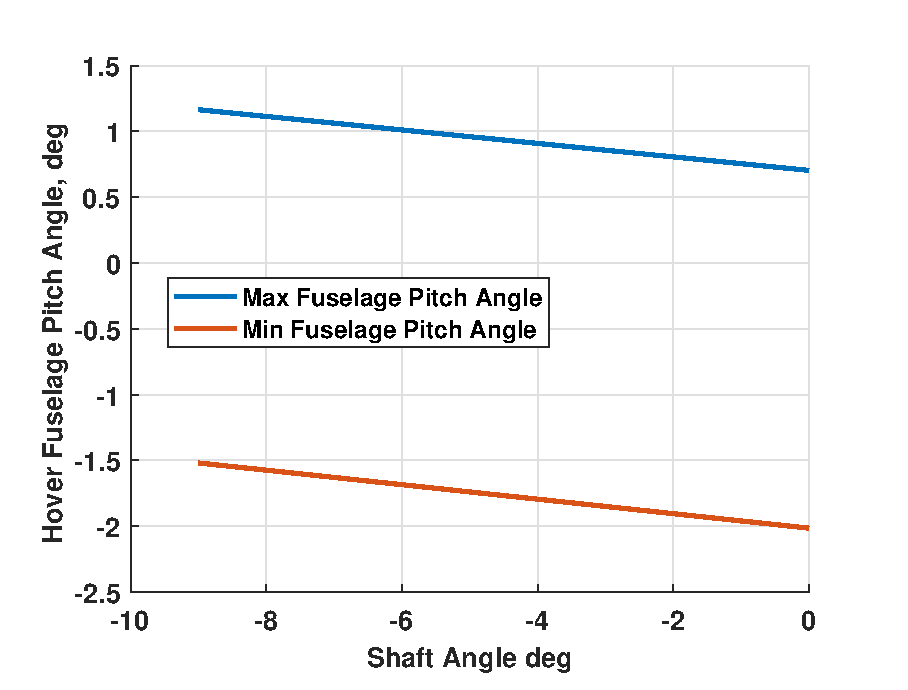
\includegraphics[width=\linewidth]{hovershaftpitch.eps}
  \captionof{figure}{Figure showing how fuselage pitch angles change with shaft tilt in hover}
  \label{fig:hshaftpitch}
\end{minipage}\hspace{0.2cm}
\begin{minipage}{.48\textwidth}
  \centering
  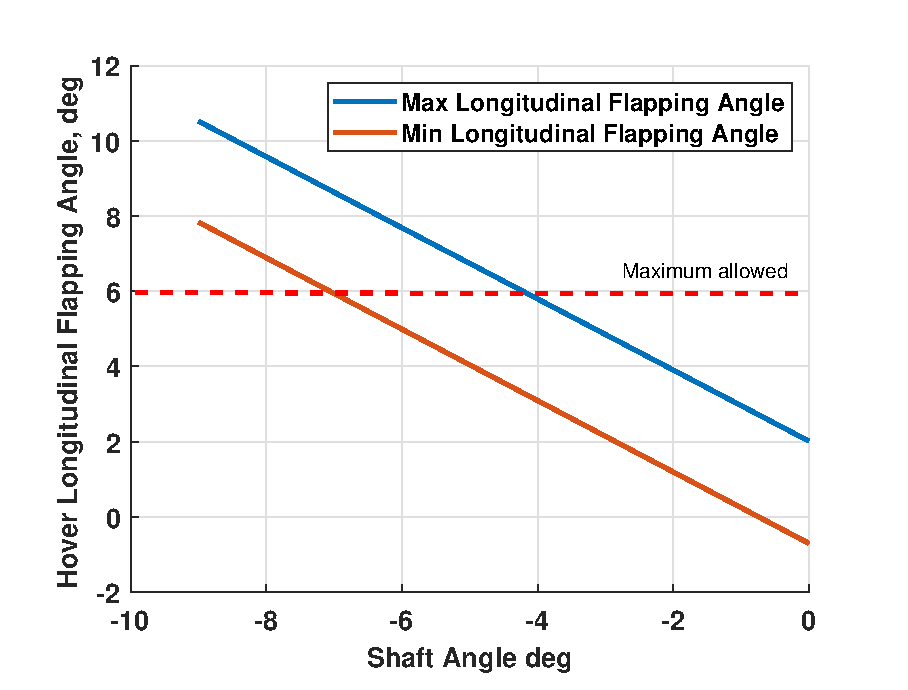
\includegraphics[width=\linewidth]{hovershaftflap.eps}
  \captionof{figure}{Figure showing how longitudinal flapping angles change with shaft tilt in hover}
  \label{fig:hshaftflap}
\end{minipage}
\end{figure}


\begin{figure}[H]
\centering
\begin{minipage}{.49\textwidth}
  \centering
  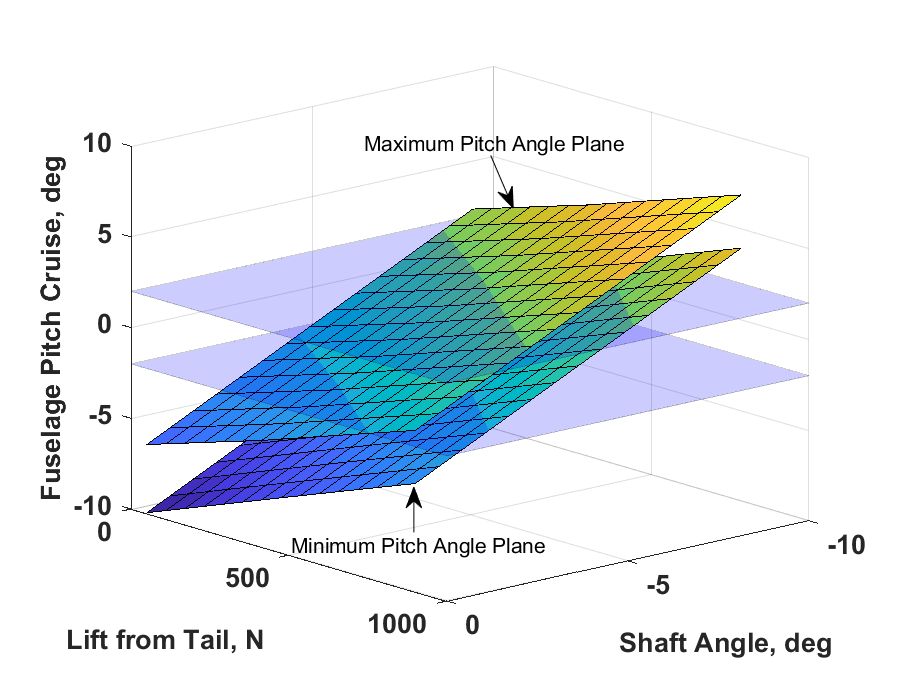
\includegraphics[width=\linewidth]{cruisepitch.eps}
  \captionof{figure}{Figure showing how cruise fuselage pitch angles change with shaft tilt  and tail force in cruise}
  \label{fig:cruisepitch}
\end{minipage}\hspace{0.2cm}
\begin{minipage}{.49\textwidth}
  \centering
  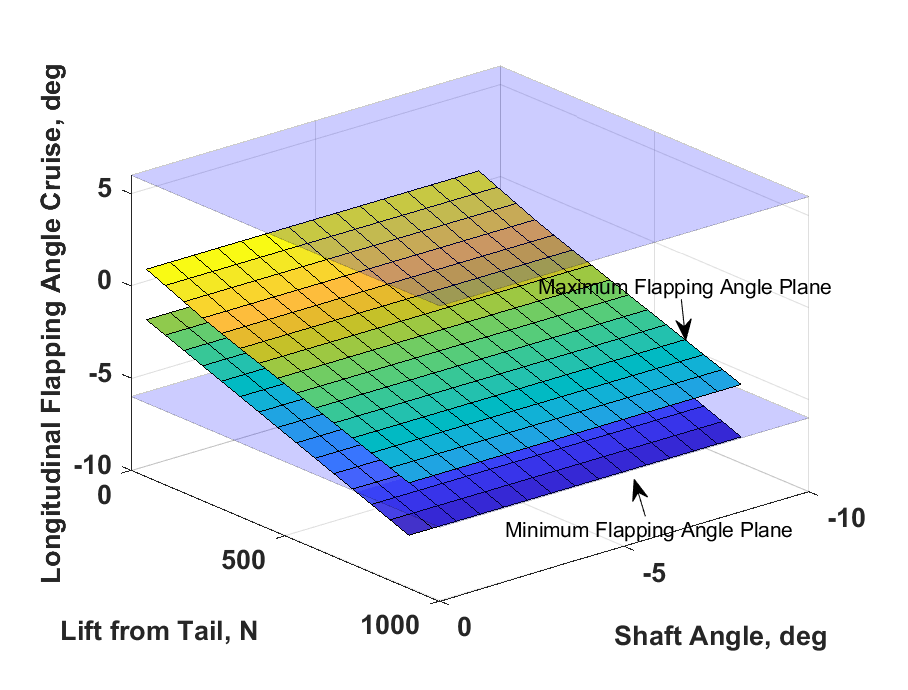
\includegraphics[width=\linewidth]{cruiseflapping.eps}
  \captionof{figure}{Figure showing how longitudinal flapping angles change with shaft tilt and tail force in cruise}
  \label{fig:cruiseflap}
\end{minipage}
\end{figure}

It is clear from the above figures that the individual relationships are approximately linear.
From Figure \ref{fig:hshaftpitch}, it can be seen that increasing the forward tilt of the rotor shaft results in increasing the nose-up pitch during hover. Figure \ref{fig:hshaftflap}, shows a similar trend with the hover flapping angle, this flapping angle proved to be the limiting factor when increasing shaft tilt.

From Figure \ref{fig:cruisepitch} it can be seen the both shaft tilt and tail force have the same effect of linearly increasing the pitch angle of the fuselage in cruise. In Figure \ref{fig:cruiseflap}, it can be seen that the shaft angle has minimal effect on the flapping angle, this is expected as during cruise the shaft tilt only serves to bring up the nose. It also shows that as $L_t$ increases the longitudinal flapping angles decreases. This trend limited the maximum $L_t$ allowed.

It is not straightforward to state that increasing a particular parameter is desirable for a certain result as it depends on the starting point from which you choose to vary.


\subsection{Configuration Selection}


Following this data gathering, the challenge was to create a method to find the best solution, or a solution that best satisfied a criteria. Many methods of optimisation were attempted that tried to minimise fuselage pitch angles while also minimising flapping angles. The method presented here is to rule out combinations of $\gamma$ and $L_t$ that resulted in values that exceeded a threshold.

To do this a criteria was formed:

\begin{itemize}
    \item A fuselage pitch angle of up to $\pm2$ degrees would be allowed in all conditions this is judged to be imperceptible to the passenger.
    \item Maximum flapping angle allowed in all conditions is $\pm6$ degrees, this is considered a large flapping angle \cite{prouty}\cite{padfield}.
\end{itemize}{}

These limitations are visualised in the above figures through boundary planes in the surface plots and dashed lines in Figure \ref{fig:hshaftflap}.
This resulted in only two out of the $225$ tested combinations satisfying the constraint:

\begin{table}[H]
\centering 
    \caption{Table showing final cases that satisfy criteria}
\begin{tabular}{ccc}
\hline
  \rowcolor[HTML]{DAE8FC} 
  Parameter & Case 1 & Case 2\\ \hline
   Shaft Tilt, $\gamma$ & $-3.86$ deg & $-3.86$ deg\\
   Tail Force, $L_t$ & $657.14N$ & $717.86N$\\
   \hline
\end{tabular}{}
    \label{tab:long}
\end{table}{}

The only differing value between the cases in Table \ref{tab:long} is the Tail Force, suggesting differing cruise characteristics. The cruise characteristics of the two cases were plotted together, Figure \ref{fig:cases} and as the relationship between the individual parameters has been observed to be linear the points were joined by a straight line.
\begin{figure}[H]
    \centering
    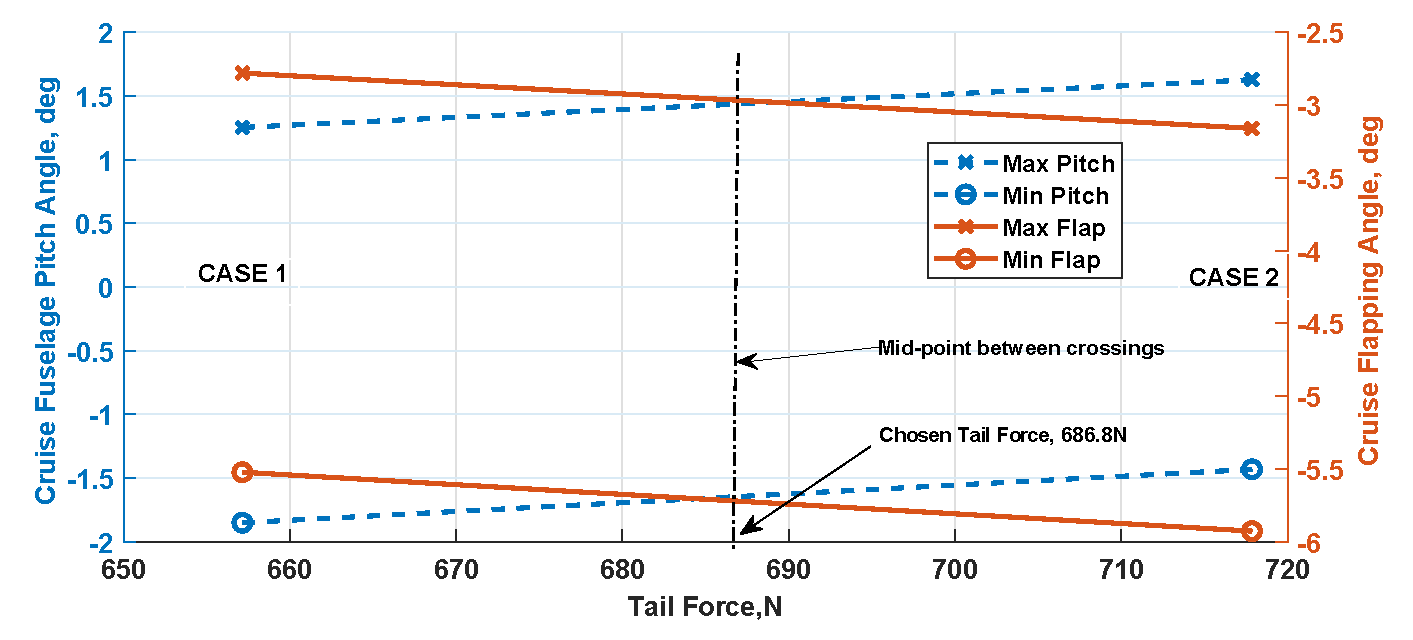
\includegraphics[width=0.9\textwidth]{cases.eps}
    \caption{Figure showing combined cruise results of both qualifying cases v. Tail Force and the final value of tail force selection method}
    \label{fig:cases}
\end{figure}{}

This plot allowed the crossings of the maximum angles and minimum angles to be found, the Tail force chosen was the mid point of these crossings which can be seen in Figure \ref{fig:cases}. This can be said to be the optimum Tail force for this shaft tilt, assuming the flapping and pitch angles are weighted equally at this stage. Thus, the final configuration is a Shaft Tilt of $\gamma=-3.86$ degrees and a Tail Force of $L_t=686.8N$.
% It was decided to optimise for minimising the delta between fuselage tilt in hover and in cruise. This allows the option the tilting seating to compensate for a near constant fuselage tilt throughout the journey. The absolute values will be checked after to ensure on ground tilt is not extreme. A surface plot of this delta, $\theta_{f_{hover}}-\theta_{f_{cruise}}$, can be seen in Figure ADDREF.

% Two points were selected along the intersection of this surface and the zero plane and were used to derive the equation of the line that represents the configurations optimised for pitch delta, $\gamma=h(L_t)$.

% Next, for each of these configurations the energy consumption due to flapping actuation were calculated and a minimum found.
% The cost function for energy is as follows:
% \begin{align}
%     \text{Energy Consumption}&=f(a_{1s_{cruise}},a_{1s_{hover}})\\
%     a_{1s_{cruise}}&=g(\gamma,L_t)\\
%     a_{1s_{hover}}&=g_h(\gamma)
% \end{align}{}
% However, as $\gamma$ and $L_t$ are now dependant variables the substitution of $\gamma=h(L_t)$ can be made leading to:
% \begin{align}
%     \text{Energy Consumption}&=f(g(h(L_t)))
% \end{align}{}
% The functions $g$ and $h$ are known but assumptions have to made to obtain a relationship for $f$. It is assumed from the mission profile that only $10\%$ of the average journey would be in hover while the other $90\%$ would be in cruise. And that as flapping actuation increases energy consumption increases linearly. Therefore, it could be said that for a typical journey:

% \begin{align}
%         \text{Energy Consumption}&\propto 0.9*a_{1s_{cruise}}+0.1*a_{1s_{hover}}
% \end{align}{}





% PLOTS

% From PLOTS it can be seen that the relationships are mostly linear.

DISCUSSION

The end result of the model is a shaft tilt angle and tailplane force.
The model results give flapping angle and fuselage pitch angles in both hover and cruise.
The criteria is that fuselage pitch should  be as small as possible (ideally 0), in all cases for comfort.
The flapping angle should also be kept to a minimum (ideally 0) to conserve power.
If both are set to zero then either the helicopter will not be able to move forward or will not be able to hover.

Percentage of time in hover. 

Minimise delta between fuselage angle in hover and cruise. If large angle for both then tilt seats to compensate.

Equation of line of intersection of planes of fuselage pitch delta and zero. Use that line and calculate energy efficiency (flapping angle). Fuel consumption based on mission. flapping in hover (*0.1) + cruise (*0.9).

\section{Vertical Stabiliser Sizing}

% Describe purpose of Vstab in coaxial. 
% Dynamic analysis required.
% Show equations, assumptions
% Show how actuation was added.

% Show resulting plots, sizing.
\begin{wrapfigure}[15]{r}{5.5cm}
    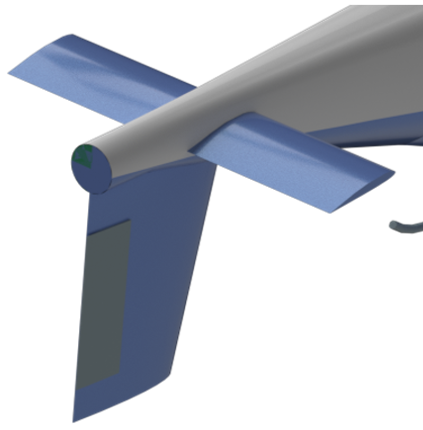
\includegraphics[width=5cm]{Empennage.png}
    \caption{SkyPass 3 Empennage }
    \label{fig:emp}
    %\vspace{-510pt}
\end{wrapfigure}
In a conventional penny-farthing helicopter the vertical stabiliser may be designed to offload the tail rotor during forward flight. However, in a coaxial helicopter where the counter-rotating rotors produce no resultant torque the vertical stabiliser plays no role in static stability. Instead, it's main purpose would be to damp out yaw disturbances through the "weather-vane" effect, increasing passenger comfort. Therefore, it was necessary to analyse the vertical stabiliser dynamically.


The design process was to create a dynamic model of the damping effects of the vertical stabiliser, use the model to obtain initial sizing for a desired damping ratio identified from literature, which is approximately 0.45 \cite{prouty}. Basic active rudder control was added to the model for comparison, allowing a decision to be made whether to opt for the actively controlled system or not for a specific damping ratio.
\subsection{Modelling}
\subsubsection{Vertical Stabiliser}
The dynamic model was created using NACA0006, chosen for its symmetry and relatively high L/D ratio and lift curve slope. The model excludes any effects of the main rotors and damping effect of the fuselage, small angles are assumed. The yaw moment of inertia of the helicopter,$I_{xy}=1118.8 kgm^2$ was used. The quarter-chord of the fin was placed $5m$ behind the CG of the helicopter ($l=5m$) to avoid downwash effects. 
\begin{figure}[H]
	\centering
	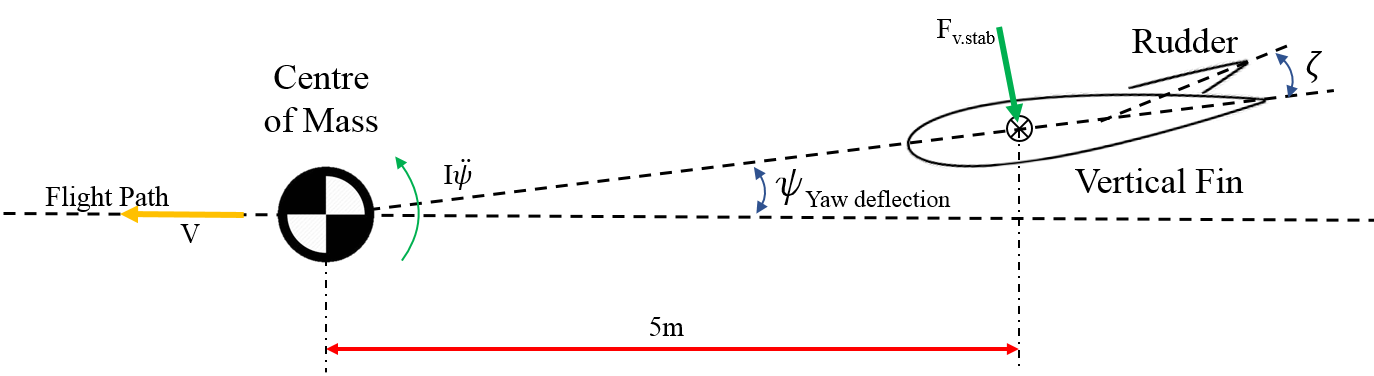
\includegraphics[width=0.9\textwidth]{VertStabdiag.PNG}
	\caption{Diagram showing model (incl. rudder)}
	\centering
	\label{fig:vertdiag}
\end{figure}

Based on the diagram in Figure \ref{fig:vertdiag}, excluding the rudder, the equation of motion was found to be:
\begin{align}
\Sigma M: I_{xy}\ddot{\psi}&=l(\frac{1}{2}\rho V^2 S_{tp}C_L(\psi+\frac{\dot{\psi}l}{V})) \\
\text{let,}\,\, A&=\frac{1}{2}\rho V^2 S_{tp}C_L\\
 \text{therefore,}\,\,I\ddot{\psi}&=\frac{Al^2}{V}\dot{\psi}+A l\psi \label{eq:eom1}
\end{align}{}

Using the Matlab tool $ode45$, Equation \ref{eq:eom1} was simulated and the damping ratio could be obtained. \\

\subsubsection{Active Rudder Control}

To observe the effects a form of active rudder control could have on the system, a few additional assumptions were made:

The deflection of the rudder is equal to the deflection of the aircraft ($\psi=\zeta$), this of course is only true for small angles. The rudder occupies a third of the area of the vertical stabiliser, this was judged to be sufficient to house the mechanism and limits the power consumption by not using the entire area. The control time delay is assumed instant, this is unrealistic but for the purposes of this project and considering the time constraints this was deemed to be a satisfactory simplification. Additionally, the difference in the location of the force generated by the rudder and by the vertical fin is assumed zero, this was judged to be a relatively valid assumption as the difference would be small relative to $l$ and in any case would generate a more conservative result. Both use the same aerofoil, ($C_{L_{tp}}=C_{L_{r}}=C_L$).

This allowed a second equation of motion to be derived, again based on Figure \ref{fig:vertdiag}:
\begin{align}{}
\Sigma M: I_{xy}\ddot{\psi}&=l(\frac{1}{2}\rho V^2 S_{tp}C_L(\psi+\frac{\dot{\psi}l}{V})+\frac{1}{2}\rho V^2 S_R C_L(\psi+\frac{\dot{\psi}l}{V}+\zeta+\frac{\dot{\zeta}l}{V})) \\
\text{let,}\,\,A&=\frac{1}{2}\rho V^2 C_L\,;\, \psi=\zeta\\
 \text{therefore,}\,\,I\ddot{\psi}&=A\,l\,\left(2\,S_{R}+\,S_{\mathrm{tp}} \right) \psi+\frac{3\,A\,l^2\,S_{\mathrm{tp}}\,}{V} \dot{\psi} \label{eq:eom2}
\end{align}{}

\subsection{Results \& Discussion}
Equations \ref{eq:eom1} and \ref{eq:eom2} were simulated in Matlab and the damping ratios for each were obtained for a range of surface areas. This can be seen in Figure \ref{fig:vstab1}.

\begin{figure}[H]
\centering
\begin{minipage}{.48\textwidth}
  \centering
  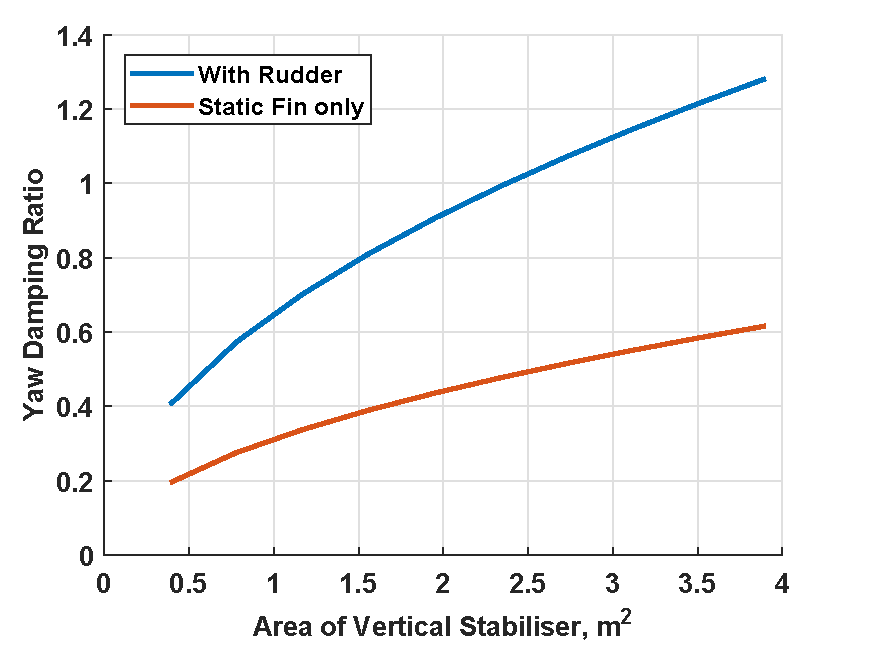
\includegraphics[width=\linewidth]{DampVArea2.eps}
  \captionof{figure}{Figure showing Damping Ratio V Area for both implementations}
  \label{fig:vstab1}
\end{minipage}\hspace{0.2cm}
\begin{minipage}{.48\textwidth}
  \centering
  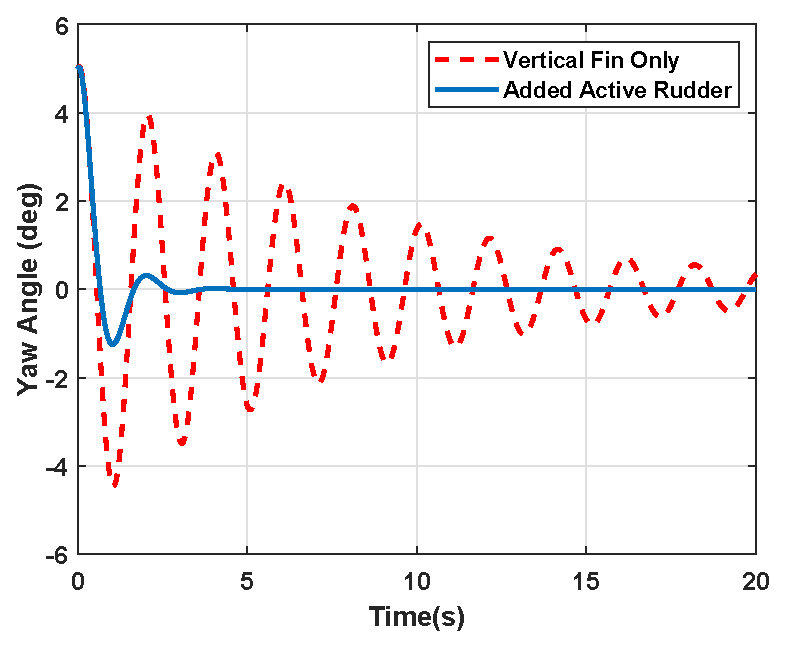
\includegraphics[width=0.9\linewidth]{Vstabresp2.eps}
  \captionof{figure}{Time Response of chosen area ($0.39m^2$), comparison with static fin}
  \label{fig:vstab2}
\end{minipage}
\end{figure}

As can be seen from Figure \ref{fig:vstab1} the active rudder offers a much greater degree of damping for the same area. The damping was increased by $2.08$ times in every case. To obtain the level of damping required, an area of $0.39m^2$ was chosen with rudder control. The time response comparison to that of no rudder and the same area can be seen in Figure \ref{fig:vstab2}.

The decision was made to have the vertical stabiliser mounted below the tail, this was to ensure that any lateral force generated by the fin would not induce a large rolling moment as the centre of pressure would be much more in line with the vertical location of CG, this can be seen in the GA. This does mean that the stabiliser could be less effective as it may be in the wake of the fuselage, however, this is less of an issue as it is not expected to be used during normal flying conditions as the aircraft employs differential torque of the rotors as its main method of yaw control. Any disturbance in yaw would increase the exposure of the stabiliser to the air and assist in damping. Another, is the case of auto-rotation, where the velocity vector is downwards meaning the stabiliser will not be blocked by the fuselage and will help in keeping the aircraft facing forward.

In all other cases, the vertical stabiliser is not considered a 'mission critical' surface, meaning it is not absolutely required to maintain normal flight in the case of a coaxial helicopter. It is implemented here to increase passenger comfort and handling.
\begin{table}[H]
\centering 
    \caption{Final Parameters of Vertical Stabiliser}
\begin{tabular}{cc}
\hline
  \rowcolor[HTML]{DAE8FC} 
  Parameter & Value  \\ \hline
   Area  & $0.39m^2$\\
   Aerofoil & NACA0006\\
   Damping Ratio & $0.404$\\
   Position from Cabin centre & $5m$\\
   \hline
\end{tabular}{}
    \label{tab:vstab}
\end{table}{}
Future work may be done to assess the rudder's use as a method of yaw control that may or may not have a energy saving effect by  reducing the role of the main rotors in this. Further, the considerations and assumptions of the models may be improved to allow more accurate data to be produced to better inform the design. Namely, a more realistic control system, effects of the fuselage and rotors during a yaw deflection could be implemented as well as model verification through wind tunnel testing.


\section{Summary and Conclusions}


%-------------------------------------------------------------------------------
% REFERENCES
%-------------------------------------------------------------------------------
\begin{thebibliography}{}
\bibitem{prouty}R. Prouty, Helicopter performance, stability, and control. Malabar: Krieger Pub., 2005.
\bibitem{padfield} Padfield, Gareth D., et al. Helicopter Flight Dynamics : the Theory and Application of Flying Qualities and
Simulation Modelling. Second ed., Blackwell Publishing, 2007
\end{thebibliography}{}
%-------------------------------------------------------------------------------
% APPENDIX
%-------------------------------------------------------------------------------

\begin{appendices}
\addcontentsline{toc}{section}{APPENDIX}
\renewcommand\thefigure{A.\arabic{figure}}  
\setcounter{figure}{0}

\begin{table}[H]
\centering
\caption{Table showing a more detailed mass breakdown}
\begin{tabular}{cc}
\hline
\rowcolor[HTML]{DAE8FC} 
Component                      & Mass (kg)                       \\ \hline
Cooling System                 & 50                              \\ \hline
Air Conditioning               & 25                              \\ \hline
Cabling                        & 55                              \\ \hline
Inverters                      & 20.4                            \\ \hline
Motors                         & 200 (50x4)                      \\ \hline
Gearbox                        & 200                             \\ \hline
Rotor Blades                   & 150.73                          \\ \hline
Rotor Hub                      & 258                             \\ \hline
Avionics                       & 120                             \\ \hline
Batteries                      & 660                             \\ \hline
Cabin Structure                & 250                             \\ \hline
Interior                       & 190.5                           \\ \hline
\textbf{Total OWE + Batteries} & \cellcolor[HTML]{FFCCC9}2179.63 \\ \hline
Payload                        & 550                             \\ \hline
\textbf{MTOW}                  & \cellcolor[HTML]{FFCCC9}2729.63 \\ \hline
\end{tabular}
\label{tab:massb}
\end{table}


\begin{figure}[H]
	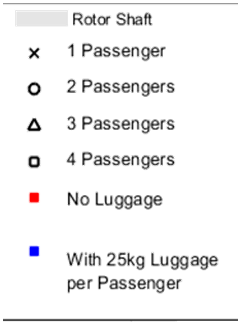
\includegraphics[width=0.2\textwidth]{Legend.PNG}
	\label{fig:batterypos}
\end{figure}



\begin{figure}[H]
\centering
\begin{minipage}{.5\textwidth}
  \centering
  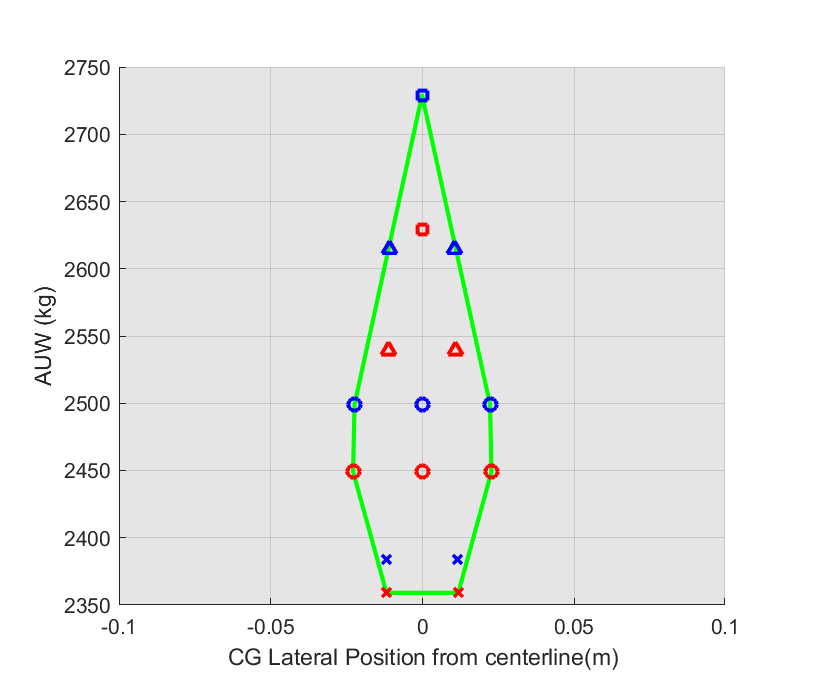
\includegraphics[width=\linewidth]{CGLAT.eps}
  \captionof{figure}{Lateral CG versus AUW}
  \label{fig:CGlat}
\end{minipage}%
\begin{minipage}{.5\textwidth}
  \centering
  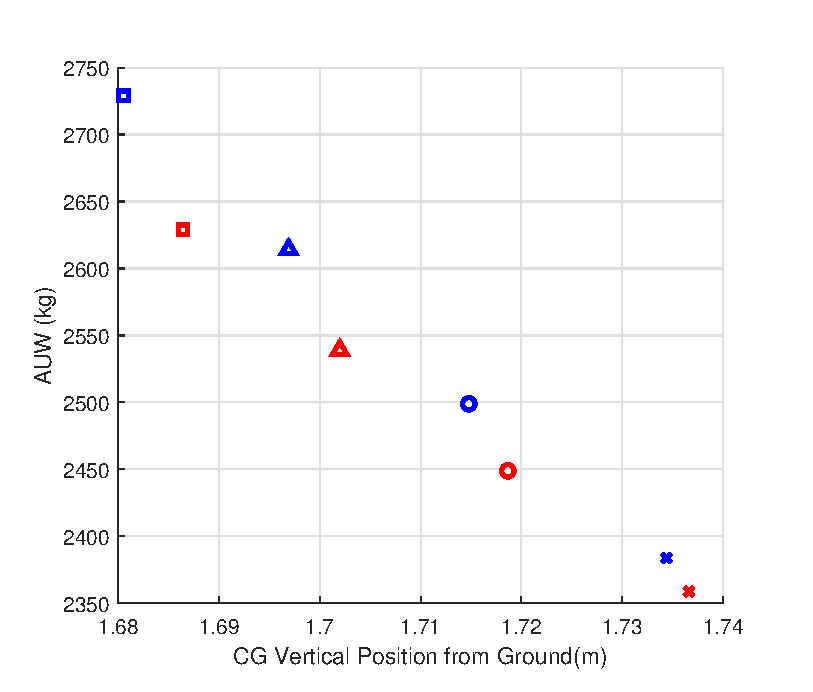
\includegraphics[width=\linewidth]{CGVERT.eps}
  \captionof{figure}{Vertical CG versus AUW}
  \label{fig:CGvert}
\end{minipage}
\end{figure}



\begin{figure}[H]
	\centering
	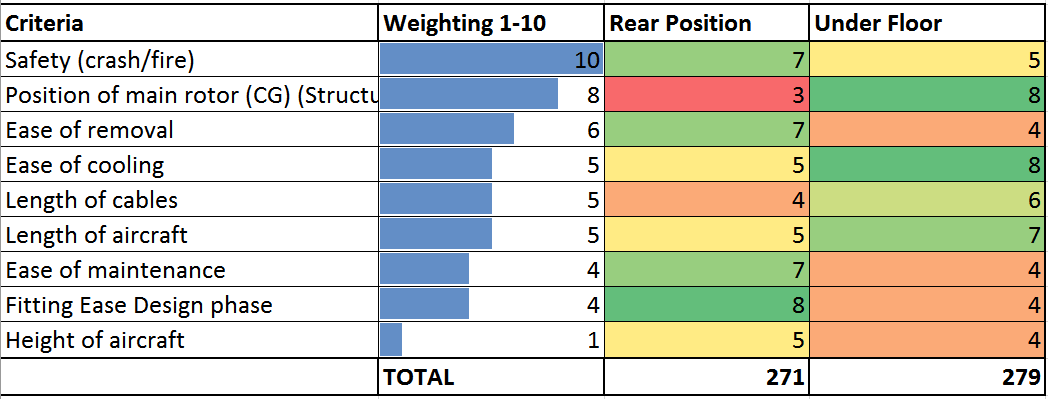
\includegraphics[width=0.8\textwidth]{batterypos.PNG}
	\caption{Trade study to decide position of battery}
	\centering
	\label{fig:batterypos}
\end{figure}
\end{appendices}{}
\end{document}

%%NOTES
%Assumption  hover is in still air
%Cruise is in still air
%

%-------------------------------------------------------------------------------
% SNIPPETS
%-------------------------------------------------------------------------------

% \begin{figure}[!ht]
% 	\centering
% 	\includegraphics[width=0.8\textwidth]{file_name}
% 	\caption{}
% 	\centering
% 	\label{label:file_name}
% \end{figure}

%\begin{figure}[!ht]
%	\centering
%	\includegraphics[width=0.8\textwidth]{graph}
%	\caption{Blood pressure ranges and associated level of hypertension (American Heart Association, 2013).}
%	\centering
%	\label{label:graph}
%\end{figure}

%\begin{wrapfigure}{r}{0.30\textwidth}
%	\vspace{-40pt}
%	\begin{center}
%		\includegraphics[width=0.29\textwidth]{file_name}
%	\end{center}
%	\vspace{-20pt}
%	\caption{}
%	\label{label:file_name}
%\end{wrapfigure}

%\begin{wrapfigure}{r}{0.45\textwidth}
%	\begin{center}
%		\includegraphics[width=0.29\textwidth]{manometer}
%	\end{center}
%	\caption{Aneroid sphygmomanometer with stethoscope (Medicalexpo, 2012).}
%	\label{label:manometer}
%\end{wrapfigure}

%\begin{table}[!ht]\footnotesize
%	\centering
%	\begin{tabular}{cccccc}
%	\toprule
%	\multicolumn{2}{c} {Pearson's correlation test} & \multicolumn{4}{c} {Independent t-test} \\
%	\midrule	
%	\multicolumn{2}{c} {Gender} & \multicolumn{2}{c} {Activity level} & \multicolumn{2}{c} {Gender} \\
%	\midrule
%	Males & Females & 1st level & 6th level & Males & Females \\
%	\midrule
%	\multicolumn{2}{c} {BMI vs. SP} & \multicolumn{2}{c} {Systolic pressure} & \multicolumn{2}{c} {Systolic Pressure} \\
%	\multicolumn{2}{c} {BMI vs. DP} & \multicolumn{2}{c} {Diastolic pressure} & \multicolumn{2}{c} {Diastolic pressure} \\
%	\multicolumn{2}{c} {BMI vs. MAP} & \multicolumn{2}{c} {MAP} & \multicolumn{2}{c} {MAP} \\
%	\multicolumn{2}{c} {W:H ratio vs. SP} & \multicolumn{2}{c} {BMI} & \multicolumn{2}{c} {BMI} \\
%	\multicolumn{2}{c} {W:H ratio vs. DP} & \multicolumn{2}{c} {W:H ratio} & \multicolumn{2}{c} {W:H ratio} \\
%	\multicolumn{2}{c} {W:H ratio vs. MAP} & \multicolumn{2}{c} {\% Body fat} & \multicolumn{2}{c} {\% Body fat} \\
%	\multicolumn{2}{c} {} & \multicolumn{2}{c} {Height} & \multicolumn{2}{c} {Height} \\
%	\multicolumn{2}{c} {} & \multicolumn{2}{c} {Weight} & \multicolumn{2}{c} {Weight} \\
%	\multicolumn{2}{c} {} & \multicolumn{2}{c} {Heart rate} & \multicolumn{2}{c} {Heart rate} \\
%	\bottomrule
%	\end{tabular}
%	\caption{Parameters that were analysed and related statistical test performed for current study. BMI - body mass index; SP - systolic pressure; DP - diastolic pressure; MAP - mean arterial pressure; W:H ratio - waist to hip ratio.}
%	\label{label:tests}
%\end{table}
